\chapter{Method}


\begin{figure}[h]
 \begin{center}
  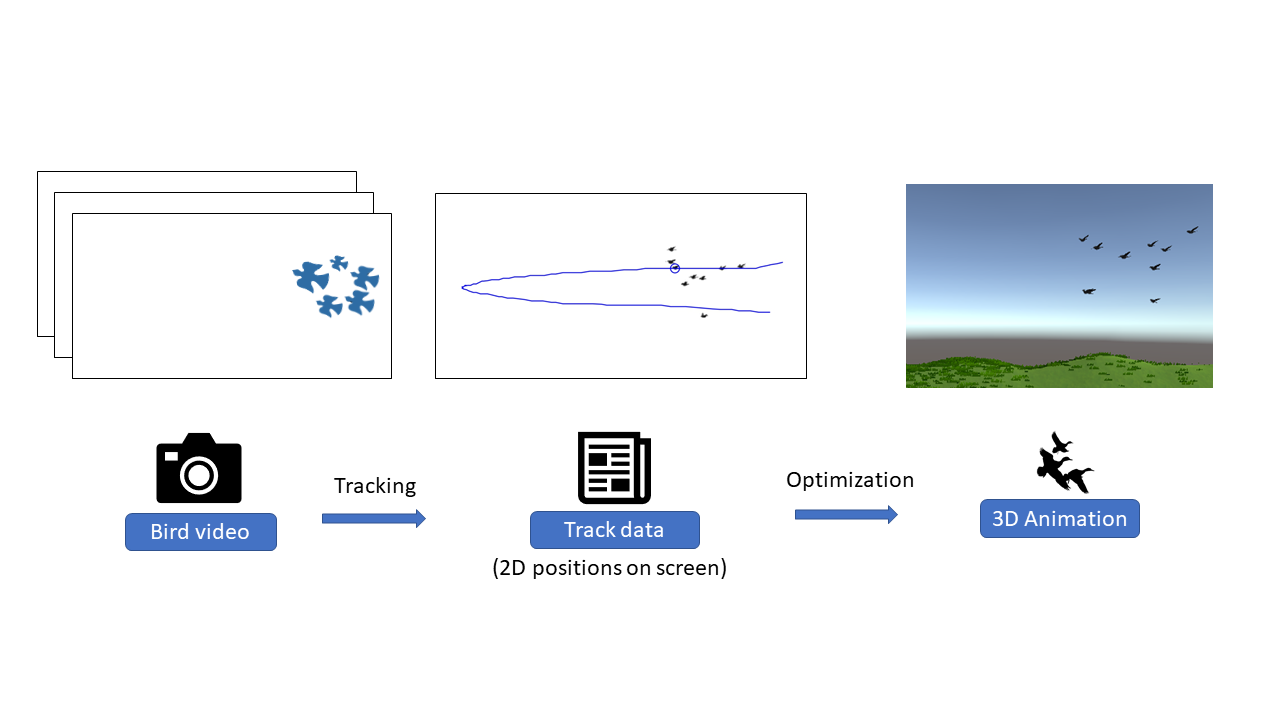
\includegraphics[width=1.0\textwidth]{system.eps}
 \end{center}
 \caption{Method overview}
 \label{figure:system}
\end{figure}


\section{Method overview}


Figure\ref{figure:system}  shows an overview of our method. As mentioned before, our method synthesizes three-dimensional bird flock motion from input video. First, trace data of each bird in the video is retrieved. With the interactive feature tracking technique, track data, which contains two-dimensional projection position trajectory of each bird, can be retrieved with the help of user's indications. Next, depth set $X$ is predicted by minimizing error function as Equation \ref{eq:1}. With the predefined camera parameter and optimal depth d, we can get world position of the bird from its screen position.
In most simulation system, velocity of an object is calculated upon mass and force in simulation steps. However, since our optimization method is over frames, we use position-based dynamics system \cite{PBD}, in which velocity in frame f is denoted as


\begin{equation}\label{eq:3}
 \vec{v(f)} = b(f)-b(f-1)
\end{equation}


where $v(f)$ denotes velocity, and $b(f)$ denotes bird position in world space. This makes our optimization system simpler and faster: we can calculate velocity of each bird in current frame and do not need to keep track of it. Although position-based dynamics system is not physically accurate, since our goal is to make visually plausible flock motion, we use it in our system.
For s and t in equation \ref{eq:2}, we use the simple Euclidean distance function on the two positions. We have also experimented with an acceleration term, of the form $s(p_n^f, p_n^{f-1}, p_n^{f-2})$, but it increases the computation cost, and do not produce better result.


\section{Bird tracking}


To obtain trajectory of each bird in the input video, tracking technique is used in our method. We use tracking system ZooTracer\cite{ZooTracer}, developed by Microsoft research, to do the task. ZooTracer is based on interactive feature tracking technique, proposed by Buchanan and Fitzgibbon \cite{Tracking}. With the tracking system, after preprocessing is done, the user can make tracking data interactively from input video in real time. The system predicts the trajectory of single bird in the video based on user's initial indication. If the tracking is wrong in some frames, user can provide keyframe features by few clicks and improve the track.
The main challenge of using interactive feature tracking on tracking birds is distinguishing between tracked birds. The system records fixed-size image patches for tracking feature points, such as eye on a face. However, in case of tracking bird flock, all birds look similar in small patches. It leads to many errors found in the result, making wrong tracking data. Therefore, more manual manipulations need to be done to get an optimal track. On average, user can complete the track data of one bird in a 200-frame video in less than 1 minute.



\section{Trajectory smoothness}


\begin{figure}[h]
 \begin{center}
  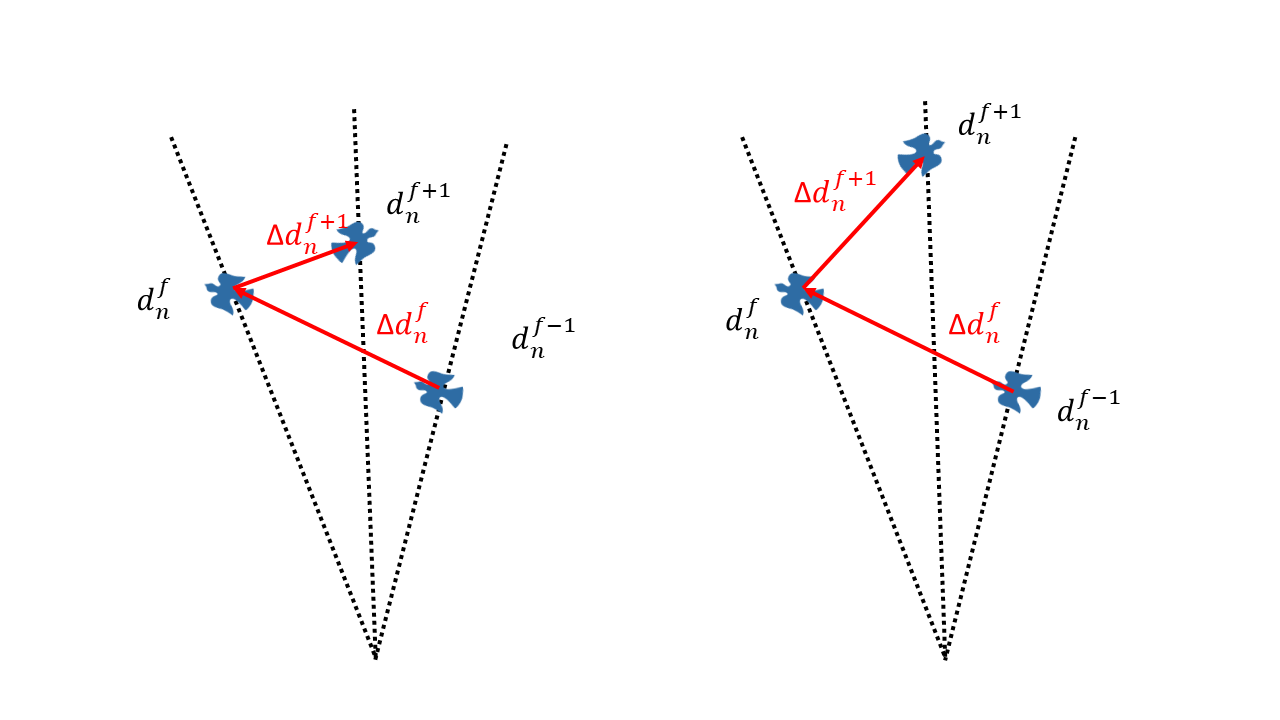
\includegraphics[width=1.0\textwidth]{turn.eps}
 \end{center}
 \caption{Trajectory smooth. Figure on the left shows the scenario of sudden turn, while the trajectory on the right is considered better trajectory, since the speed difference is smaller.}
 \label{figure:turn}
\end{figure}



Trajectory smoothness is the first term in our error function in equation \ref{eq:1}, denoted as $t(.)$. In this term, only the flying trajectory of one bird is considered. We assume that birds minimize its velocity change during flight. The importance of retaining trajectory smoothness is especially obvious when bird is on turning point of the track. In our experiment, we found that if trajectory smooth is not considered, birds will show a sudden turn motion, which is unnatural. Figure \ref{figure:turn} shows the scenario of sudden turn. Trajectory smoothness term is then denoted as:

\begin{equation}\label{eq:4}
 t(p_n^f, p_n^{f-1},d_n^f) = v_n^f = b_n^f-b_n^{f-1}
\end{equation}

as error function to be minimized in optimization stage to retain trajectory smoothness.

%where $b_f^n$ denotes projected bird position respecting to track position $p_f^n$ and depth $d_f^n$ . By combining these two terms, we can obtain:
%\begin{equation}\label{eq:6}
%t(p_n^f, p_n^{f-1},d_n^f) = \lambda_d|{|\Delta}d_n^f||+\lambda_v||{\Delta}v_n^f||
%\end{equation}


\section{Flock behavior similarity}


\begin{figure}[h]
 \begin{center}
  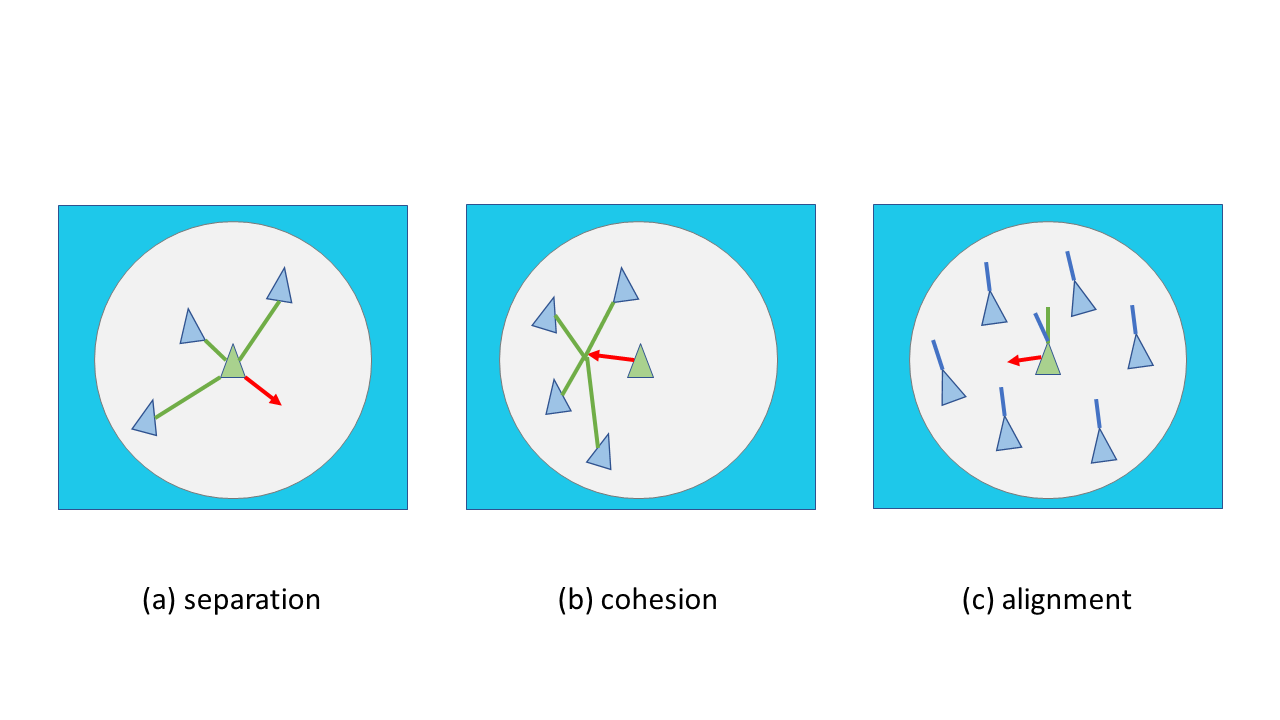
\includegraphics[width=1.0\textwidth]{boid.eps}
 \end{center}
 \caption{Three boid rules. (left) separation behavior, (middle) Cohesion behavior, (right) alignment behavior.}
 \label{figure:boid}
\end{figure}


We use Reynolds' boid model as basic flock behaviors. Each bird in flock, which is called boid, observes three steering rules: separation, cohesion, and alignment. The definitions of these steering rules rely on the neighbors of the boid. The neighbors of one boid include its surrounding neighbors who are sufficiently close, and each rule has its perceptual neighborhood. Figure \ref{figure:boid} illustrates the definition of three rules. To calculate flock similarity, target position of boid $n$ in frame $f$ must be calculated first, and then compared with the predicted boid position. Target position is the sum of the three rules above. Here we further the calculation of three steering rules.


Separation steering behavior gives a boid the ability to maintain a certain separation distance from others nearby and to prevent boids from crowding together. We think that separation rule is the most important rule for creating nature flock motion, since collision with other birds is obviously unnatural. To compute separation force, first a search is made to find other boids within the specified neighborhoods. For each nearby boid, the force is computed by subtracting the positions of the boid and the nearby boids, normalizing, and then applying a $1/r$ weighting, making force of nearer nearby boid stronger. All forces for each nearby boid are summed together to produce the overall separation force.


Cohesion steering behavior give a boid the ability to approach and form a group with other nearby characters. That is, boids steer towards the average position of the nearby boids. This behavior helps flock to form a group and not be too separated. The neighborhood of cohesion is set much bigger than neighborhood of separation does to keep the flock form in group while preventing collision.


Alignment steering behavior gives a boid the ability to align itself, heading in the same direction with other nearby boids. However, since in the optimization stage, we only consider optimizing position of each boid, we do not use alignment rule here. Instead, we refine the alignment after optimization is done.


\begin{algorithm}[p]
\SetAlgoLined
\tcp{Calculate separation force $\vec{s}$ of bird n}
$\vec{s} \leftarrow \vec{0}$ \;
$neighbor \leftarrow 0 $ \;
\For{$i\leftarrow 1$ \KwTo $N$}{
  \lIf{i=n}{continue}
  $distance \leftarrow ||b_n - b_i||$ \; 
  \If{distance $\leq d_{sep}$}{
    $neighbor \leftarrow neighbor+1$ \;
    $\vec{s} \leftarrow \vec{s} + (b_n - b_i) / distance$ \;
  }
}
$\vec{s} \leftarrow \vec{s} / neighbor$ \;
\caption{Calculation of separation vector $\vec{s}$}
\label{algo:separation}
\end{algorithm}


\begin{algorithm}[p]
\SetAlgoLined
\tcp{Calculate cohesion force $\vec{c}$ of bird n}
$\vec{c} \leftarrow \vec{0}$ \;
\For{$i\leftarrow 1$ \KwTo $N$}{
  \lIf{i=n}{continue}
  $\vec{c} \leftarrow \vec{c} + (b_i - b_n)$ \;
}
$\vec{c} \leftarrow \vec{s} / (n-1)$ \;
\caption{Calculation of cohesion vector $\vec{c}$}
\label{algo:coherence}
\end{algorithm}


Combining rules above, now we can calculate flock behavior similarity term $f(.)$ in equation \ref{eq:2} by calculating Euclidean distance between the target position and predicted position. Algorithm of calculating separation and cohesion are shown in Algorithm \ref{algo:separation} and \ref{algo:coherence}.
In most flock simulation approaches, collision is detected in advance by adjusting its direction and speed when other agents are about to collide. In our flock model, since we have separation rule that separate, birds tend to move away to each other when they are too close. Therefore, we do not handle collision avoidance.


\section{Optimization}

\begin{algorithm}% [H]
\SetAlgoLined
\KwData{Trace set $X=\big\{d_n^f\big\}$}
%\KwResult{how to write algorithm with \LaTeX2e }
\tcp{Algorithm start}
Assign N bird positions in frame 1 \;
\tcp{Frame-by-frame optimization}
\For{$i\leftarrow 2$ \KwTo $F$}{
  $sum \leftarrow 0$ \;
  \tcp{Initial speed}
  \For{$j\leftarrow 1$ \KwTo $N$}{
    $\vec{v} \leftarrow b_j^i - b_j^{i-1}$ \;
    \If{i = 2}{
      $sum\leftarrow sum + || ||\vec{v}|| - \lambda_{speed}||$ \;
    }
    \Else{
      \tcp{Trajectory smoothness}
      $\vec{v_{last}} \leftarrow b_j^{i-1} - b_j^{i-2}$ \;
      $sum\leftarrow sum + \lambda_{t}|| ||\vec{v}|| - ||\vec{v_{last}}||  ||$ \;      
      \tcp{Flock behavior similarity}
      Calculate separation force $\vec{s}$ \;
      Calculate cohesion force $\vec{c}$ \;
      $target \leftarrow b_j^{i-1} + (w_{sep} \vec{s}+(1-w_{sep})\vec{c})$ \;   
      $sum\leftarrow sum + \lambda_{f}|| b_j^i - target  ||$ \; 
    }
  }
  Minimize $sum$ \;
}

\caption{Optimization algorithm detail.}
\label{algo:optimization}
\end{algorithm}



The task in our optimization stage is to minimize error function equation \ref{eq:1} with target depth set $X$. Totally, since we have track data of $N$ birds in $F$ frames, there are $N{\times}F$ target depths. If the optimization is done globally, the computation time will be costly. Since our goal is to make system that user can adjust the result interactively in real time, we consider doing the optimization frame-by-frame.
Frame-by-frame optimizations means we do not do the optimization in one equation, instead, we predict $N$ depths in frame $f$ from the first frame to next frame, based on the results from last frames. This approach greatly decreases computation time, making it possible for user to do the optimization repeatedly while adjusting parameters.
We implement the optimization part using NLopt library \cite{NLopt} with optimization algorithm constrained optimization by linear approximation (COBYLA)\cite{COBYLA}. We assume bird flock fly in an area in view field of the camera, a near and a far constraint of depth is set as:


\begin{equation}\label{eq:depth}
d_{near} < d < d_{far}
\end{equation}

Since target error function can be calculated in each frame, with the inequality constraint \ref{eq:depth}, optimized $X$ can be found as result.  Algorithm \ref{algo:optimization}  shows our optimization algorithm.
(TODO:OPTIMIZATION DETAIL)


By now, we have introduced 5 parameters for optimization stage: $\lambda_{t}$ for weight of trajectory smoothness, $\lambda_{f}$ for weight of flock behavior similarity, $\lambda_{sep}$ for weight of separation rule, $d_{near}$ for near constraint of depth and $d_{far}$ for far constraint. In our system, these parameters are treated as interactive elements of our system. Since the optimization can be done in seconds, user can see the result and adjust parameter can do the optimization again to get better results. 


\section{Modeling flock motion}


After we get the optimized depth data, next step is to visualize the optimized flock motion. We implement it with Unity\cite{Unity}. And optimization system is loaded as plugin to make it can be used in an interactive way.
After the position of each bird in every frame is predicted, to make good flock motion, refinement must be done. Since the system only finds optimal position of each bird, orientation needs to be assigned to complete flock motion. Here we just simply decide orientation of each bird frame-by-frame based on its current position and position in last frame.
(TODO:MODELING DETAIL)
